\section{Diffusion Model}
1. \textbf{Forward Process (+ Noise):} \\
   \[
   q(x_t|x_{t-1}) = \mathcal{N}(x_t; \sqrt{1-\beta_t} \cdot x_{t-1}, \beta_t \cdot I)
   \] \\
   Adding noise at each time step. \\
2. \textbf{Backward Process (Denoising):} \\
   \[
   p(x_{t-1}|x_t) \propto p_0(x_t|x_{t+1}) \prod_{t=1}^T q(x_t|x_{t-1})
   \] \\
   \[
   p_0(x_{t+1}, x_t) = \mathcal{N}(x_t; \mu(x_t, t), \sigma(x_t, t))
   \] \\
   Iteratively denoising until the original data is reconstructed.

3. \textbf{Generative Models:} \\
   a. \textbf{VAE:} Maximize the variational lower bound. \\
   b. \textbf{GAN:} Adversarial training. \\
   c. \textbf{Diffusion Model:} Add noise and then remove it. \\

4. \textbf{Time Embedding for DDPM-UNet:} fed to each layer. \\

5. \textbf{Score-Based SDE Perspective:} \\
   a. Forward process as a stochastic differential equation: \\
      \[
      x_t = x_{t-1} - \frac{\beta(t)}{2} \cdot \Delta t + \sqrt{\beta(t)} \cdot \mathcal{N}(0, I)
      \] \\
      \[
      dx = - \frac{\partial \beta(t)}{\partial x} \cdot \Delta t + \sqrt{\beta(t)} \cdot dw
      \] \\

6. \textbf{Latent Diffusion Model (Stable Diffusion):} \\
   a. LDM: Autoencoder + latent diffusion model (U-Nets) + conditional encoders. \\
   b. \textbf{Applications:} \\
      Image generation, Text-to-image generation, Semantic synthesis, Super-resolution, Inpainting. \\

    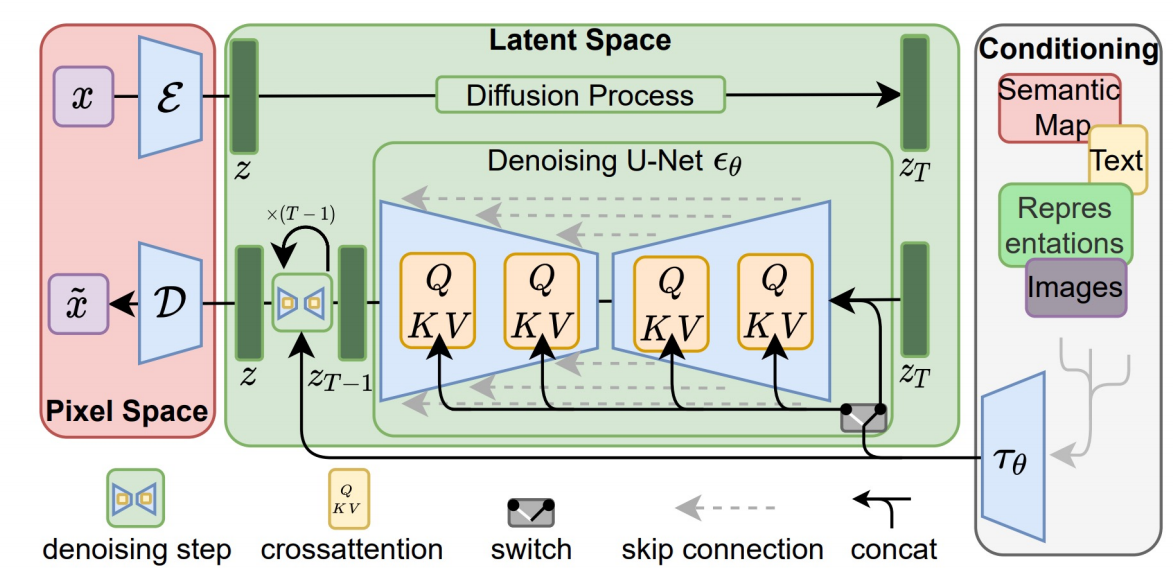
\includegraphics[width=1\linewidth]{images/latent-diff.png}
    
7. \textbf{Video Diffusion Model:} \\
   a. Direct training on video (e.g., Video LDM). \\
   b. Pretrained text-to-image model (e.g., Text2Video-Zero). \\
   c. Pretrained model + training on video motion (e.g., Animate-Diff). \\